\documentclass[conference,10pt]{IEEEtran}
\usepackage[utf8]{inputenc}
\usepackage[T1]{fontenc}
\usepackage[spanish,es-noshorthands,es-tabla]{babel}
\usepackage{amsmath,amssymb}
\usepackage{graphicx}
\usepackage{booktabs}
\usepackage{multirow}
\usepackage{tikz}
\usetikzlibrary{arrows.meta,positioning,fit}
\usepackage{listings}
\usepackage{xcolor}
\usepackage[hidelinks]{hyperref}
\usepackage{url}
\usepackage{cite}
\usepackage{multicol}

% Cifras generadas a partir de runs/summary.json (analisis/aggregate.py)
\newcommand{\ExpTotal}{11}
\newcommand{\EAgoals}{18.6}
\newcommand{\EAgoalsAgainst}{0.0}
\newcommand{\ECscores}{0--30, 0--35 y 0--23}
\newcommand{\LocN}{295\,889}
\newcommand{\VideoDur}{3:44~min}


\lstdefinestyle{code}{basicstyle=\ttfamily\fontsize{6.3}{7.2}\selectfont,
  breaklines=true, columns=fullflexible, keepspaces=true, showstringspaces=false,
  commentstyle=\color{black!55}, keywordstyle=\bfseries, numbers=left,
  numberstyle=\tiny\color{black!40}, numbersep=4pt, frame=none, xleftmargin=8pt,
  literate={á}{{\'a}}1 {é}{{\'e}}1 {í}{{\'i}}1 {ó}{{\'o}}1 {ú}{{\'u}}1 {ñ}{{\~n}}1
           {Á}{{\'A}}1 {É}{{\'E}}1 {Í}{{\'I}}1 {Ó}{{\'O}}1 {Ú}{{\'U}}1 {Ñ}{{\~N}}1
           {º}{{$^{\circ}$}}1 {¿}{{?`}}1 {¡}{{!`}}1 {·}{{$\cdot$}}1 {→}{{$\to$}}1
           {±}{{$\pm$}}1 {×}{{$\times$}}1}
\lstset{style=code}
\renewcommand{\lstlistingname}{Listado}

\begin{document}

\title{Validación de jugadores virtuales autónomos en RoboCup Soccer Simulation 2D: avance del proyecto final}

\author{\IEEEauthorblockN{[Nombre del estudiante 1], [Nombre del estudiante 2]}
\IEEEauthorblockA{[Programa académico] -- [Universidad]\\
{[Ciudad]}, Colombia\\
\{correo1, correo2\}@[dominio]}}

\maketitle

\begin{abstract}
Este avance documenta la puesta en marcha del servidor oficial RoboCup Soccer
Simulation 2D (\texttt{rcssserver} 19.0.0) y la implementación de
\emph{AutonomoFC}, un equipo de once agentes escrito desde cero en Python que
se comunica con el servidor por UDP, se auto-localiza triangulando banderas del
campo y decide con una formación 4-3-3 dinámica, selección de interceptor por
tiempo de llegada y un árbol de decisión tiro--pase--conducción--despeje. Se
definen métricas de equipo, de agente y de calidad interna (error de
localización, tiempo de cómputo) y se reportan resultados preliminares de
\ExpTotal{} partidos completos: AutonomoFC vence a una línea base reactiva con
un promedio de \EAgoals{} goles a favor y \EAgoalsAgainst{} en contra, pero
pierde frente a HELIOS-base (\ECscores), lo que delimita el trabajo restante.
\end{abstract}

\begin{IEEEkeywords}
RoboCup, simulación 2D, sistemas multiagente, agentes autónomos, auto-localización.
\end{IEEEkeywords}

\section{Introducción}
La liga de simulación 2D de RoboCup modela un partido de fútbol entre dos
equipos de once agentes autónomos que solo perciben el entorno de forma
parcial y ruidosa, y actúan mediante comandos discretos cada ciclo de
100~ms \cite{rcssmanual}. El objetivo de esta entrega es validar el
comportamiento de jugadores virtuales propios en ese entorno: (i) evidenciar
el servidor en funcionamiento, (ii) implementar un agente con estrategias
autónomas distinto de los clientes de ejemplo, (iii) definir métricas de
evaluación, y (iv) registrar los problemas encontrados y los siguientes pasos.

\section{Entorno de simulación}
El servidor se compiló desde el repositorio oficial \cite{rcssserver}
(\texttt{rcssserver-19.0.0}, commit \texttt{ce87001}) con CMake, Boost y
flex/bison en Ubuntu~24.04; el visor \texttt{rcssmonitor} 19.0.1 se compiló
con Qt5 \cite{rcssmonitor}. El Listado~\ref{lst:server} muestra la salida
real del servidor al cerrar un partido de evaluación y la Fig.~\ref{fig:monitor},
una captura del monitor reproduciendo un partido de AutonomoFC.

\lstinputlisting[float=t,caption={Salida del servidor (extracto, partido E1, semilla 1).},label=lst:server,numbers=none,basicstyle=\ttfamily\fontsize{6.3}{7.2}\selectfont]{evidencia_servidor.txt}

\begin{figure}[t]
\centering
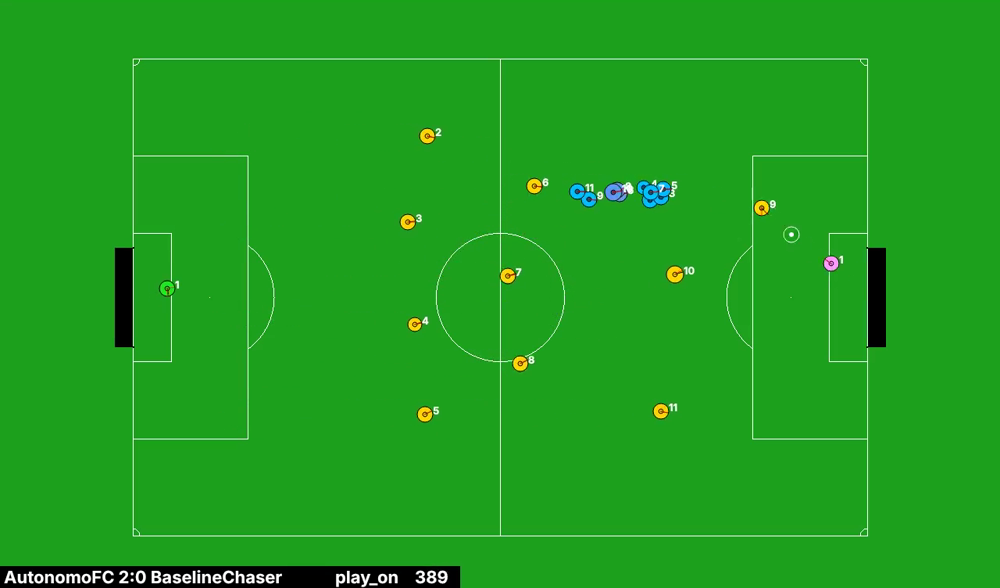
\includegraphics[width=\columnwidth]{fig/monitor.png}
\caption{\texttt{rcssmonitor} reproduciendo el log \texttt{.rcg} del partido
E1 (ciclo 389): AutonomoFC (amarillo) conserva su formación 4-3-3 mientras
BaselineChaser (azul) se amontona sobre el balón.}
\label{fig:monitor}
\vspace{-1em}
\end{figure}

Para las evaluaciones se usa el modo sincrónico (\texttt{server::synch\_mode=true}):
el servidor avanza en cuanto todos los clientes envían \texttt{(done)}, lo que
permite jugar un partido completo de $2\times3000$ ciclos en 1--3~min sin alterar
la física. El video de demostración se obtiene reproduciendo los logs del
servidor en el monitor oficial. Se usan los parámetros por defecto, sin
entrenador; el servidor asigna tipos de jugador heterogéneos con la semilla
\texttt{player::random\_seed}, distinta en cada partido.

\section{Agente propuesto: AutonomoFC}
Cada jugador es un proceso independiente (Fig.~\ref{fig:arq}) que se conecta
al puerto 6000 con el protocolo versión 19 y repite, cada vez que recibe
\texttt{sense\_body}, el ciclo percepción--modelo--decisión--acción. No se
usa información global del servidor ni comunicación entre agentes: toda la
coordinación surge de que cada agente aplica las mismas reglas sobre su
propia percepción.

\begin{figure}[t]
\centering
\begin{tikzpicture}[font=\scriptsize, node distance=3mm and 7.5mm,
  box/.style={draw, rounded corners=1.5pt, align=center, minimum height=7mm, inner sep=2pt, fill=black!4},
  >={Stealth[length=1.6mm]}]
\node[box] (srv) {Servidor\\\texttt{rcssserver}};
\node[box, right=of srv] (parse) {Parser\\S-expr.};
\node[box, right=of parse] (wm) {Modelo del\\mundo};
\node[box, right=of wm] (dec) {Decisión\\rol +\\árbol};
\draw[->] (srv) -- node[above,font=\tiny]{UDP} (parse);
\draw[->] (parse) -- (wm);
\draw[->] (wm) -- (dec);
\draw[->] (dec.south) -- ++(0,-4mm) -| node[pos=0.25,below]{\texttt{dash, turn, kick, catch, turn\_neck, move}} (srv.south);
\end{tikzpicture}
\caption{Arquitectura de cada agente (un proceso por jugador).}
\label{fig:arq}
\vspace{-1em}
\end{figure}

\subsection{Percepción y auto-localización}
El mensaje \texttt{see} entrega, para cada bandera visible, distancia $d$ y
dirección $\alpha$ relativas a la cabeza. Para cada par de banderas $A,B$
con vectores relativos $\mathbf r_A,\mathbf r_B$ se estima el ángulo global de
la cabeza y luego la posición:
\begin{align}
\theta&=\operatorname{atan2}(B-A)-\operatorname{atan2}(\mathbf r_B-\mathbf r_A),\\
\mathbf p&=\textstyle\sum_i w_i\,(F_i-R_\theta\,\mathbf r_i),
\end{align}
promediando $\theta$ de forma circular sobre los pares bien condicionados y
ponderando cada bandera con $w_i\propto 1/(1+d_i)$, porque el ruido de
cuantización crece con la distancia. Si el equipo juega por la derecha se
invierte la tabla de 55 banderas, de modo que el agente siempre ataca hacia
$+x$. Entre observaciones (\texttt{see} llega cada 2 ciclos en vista normal
sincronizada) se integra por odometría con la velocidad de \texttt{sense\_body}
y el giro comandado. El balón se propaga con el decaimiento del servidor
($v_{t+1}=0.94\,v_t$) y su velocidad se estima con
\texttt{distchg}/\texttt{dirchg}.

\subsection{Estrategias de decisión}
\textbf{Formación dinámica.} Cada dorsal tiene una posición base 4-3-3 que se
desplaza con el balón: $x=x_b+0.55\,x_{bal}$, $y=0.9\,y_b+0.25\,y_{bal}$. Los
defensas no superan al balón en más de 5~m y los delanteros se mantienen
1~m detrás de la línea de fuera de juego estimada (penúltimo rival visto).

\textbf{Selección de interceptor.} Cada agente predice la trayectoria del
balón y calcula el primer ciclo $n$ en que puede alcanzarlo; solo persigue el
balón si ningún compañero visible llega al menos 1.5 ciclos antes. Esto evita
el ``enjambre'' típico de los equipos reactivos.

\textbf{Árbol con balón.} (1) \emph{Tiro} si la distancia al arco es
$<22$~m, al poste opuesto al portero rival; (2) \emph{pase} si hay presión
(rival a $<5$~m), un balón parado propio, o un compañero claramente mejor
ubicado: se evalúa cada compañero entre 5 y 32~m con un criterio de avance,
espacio libre del receptor y un cono de intercepción (rival a menos de
$1.5+0.35\,s$~m de la línea a la distancia $s$); (3) \emph{despeje} en el
tercio defensivo bajo presión; (4) \emph{conducción} con toques de
0.85~m/ciclo en la dirección (entre $\pm60^\circ$) que maximiza avance y
distancia al rival más cercano. La potencia de pateo se calcula invirtiendo el
modelo del servidor (\texttt{kick\_power\_rate} con penalización por ángulo y
distancia al balón).

\textbf{Sin balón.} Marcaje: en campo propio, defensas y medios cubren al
rival más peligroso cerca de su zona, interponiéndose hacia el arco.
\textbf{Portero:} se ubica sobre la bisectriz balón--arco a $1.5$--$5$~m de
la línea, ataja (\texttt{catch}) dentro del área y saca con pase seguro o hacia
la banda. \textbf{Estamina:} la potencia de carrera se limita a 70 y 40 por
debajo de 4500 y 3000 unidades, y los no interceptores trotan si están a
menos de 8~m de su posición. \textbf{Visión:} el cuello sigue el balón o
barre $\pm90^\circ$ cuando se pierde. Tras sacar un balón parado el agente no
vuelve a tocarlo (falta por doble toque).

\subsection{Equipos de comparación}
\emph{BaselineChaser} es una línea base propia con la misma percepción pero
decisión reactiva: todos persiguen el balón y patean al arco a máxima
potencia, lo que aísla el efecto de la capa de decisión.
\emph{HELIOS-base} \cite{helios}, compilado con \texttt{librcsc}, es el equipo
de referencia abierto de la comunidad y sirve como cota superior.

\section{Métricas de evaluación}
La Tabla~\ref{tab:metricas} resume las métricas, todas calculadas
automáticamente desde el log del servidor (\texttt{.rcg}, verdad de terreno)
y los registros propios de cada agente (\texttt{analisis/metrics.py}). Un
pase se cuenta como completado cuando el siguiente toque de balón (detectado
por el contador de \texttt{kick} del servidor con el jugador a menos de
1.25~m del balón) es de un compañero; un tiro, cuando el balón sale a más de
1.6~m/ciclo hacia la boca del arco desde $x>30$.

\begin{table}[t]
\caption{Métricas para evaluar a cada agente y al equipo}
\label{tab:metricas}
\centering
\footnotesize
\setlength{\tabcolsep}{3pt}
\begin{tabular}{@{}p{1.0cm}p{3.1cm}p{3.8cm}@{}}
\toprule
Nivel & Métrica & Qué valida \\
\midrule
\multirow{4}{*}{Equipo} & Goles a favor/en contra & Eficacia global \\
 & Posesión (\%) & Control del balón (último en tocarlo) \\
 & Balón en campo rival (\%) & Dominio territorial \\
 & Tiros y tiros al arco & Generación de ocasiones \\
\midrule
\multirow{4}{*}{Agente} & Precisión de pase (\%) & Calidad de la evaluación de pases \\
 & Distancia recorrida (m) & Movilidad / posicionamiento \\
 & Estamina mínima media & Gestión de energía \\
 & Fueras de juego, faltas & Respeto de reglas \\
\midrule
\multirow{3}{*}{Interna} & Error localización P50/P90 & Calidad del modelo del mundo \\
 & Error orientación P50 & Calidad del modelo del mundo \\
 & Tiempo de decisión (ms) & Viabilidad en tiempo real \\
\bottomrule
\end{tabular}
\vspace{-1em}
\end{table}

\section{Resultados preliminares}
Se jugaron \ExpTotal{} partidos completos: E1, AutonomoFC por la izquierda
contra BaselineChaser (5 semillas); E2, lados invertidos (3 semillas), para
comprobar que la inversión de coordenadas funciona; y E3, contra HELIOS-base
(3 semillas). La Tabla~\ref{tab:res} y la Fig.~\ref{fig:res} muestran
media~$\pm$~desviación.

\begin{table*}[t]
\caption{Resultados preliminares: AutonomoFC (A) frente al rival (R), media $\pm$ desviación}
\label{tab:res}
\centering
\footnotesize
\setlength{\tabcolsep}{4pt}
\begin{tabular}{@{}lcccccc@{}}
\toprule
  & \multicolumn{2}{c}{E1: BaselineChaser (n=5)} & \multicolumn{2}{c}{E2: BaselineChaser (n=3)} & \multicolumn{2}{c}{E3: HELIOS-base (n=3)} \\
\cmidrule(lr){2-3}\cmidrule(lr){4-5}\cmidrule(lr){6-7}
Métrica & A & R & A & R & A & R \\
\midrule
Marcadores & \multicolumn{2}{c}{22-0, 18-0, 17-0, 15-0, 21-0} & \multicolumn{2}{c}{19-0, 16-2, 16-0} & \multicolumn{2}{c}{0-30, 0-35, 0-23} \\
Goles & 18.6$\pm$2.6 & 0.0$\pm$0.0 & 17.0$\pm$1.4 & 0.7$\pm$0.9 & 0.0$\pm$0.0 & 29.3$\pm$4.9 \\
Posesión (\%) & 76$\pm$2 & 24$\pm$2 & 76$\pm$1 & 24$\pm$1 & 33$\pm$5 & 67$\pm$5 \\
Balón en campo rival (\%) & 81$\pm$3 & 19$\pm$3 & 81$\pm$5 & 19$\pm$5 & 12$\pm$3 & 88$\pm$3 \\
Tiros & 23.6$\pm$4.4 & 0.2$\pm$0.4 & 21.0$\pm$0.8 & 0.3$\pm$0.5 & 0.0$\pm$0.0 & 36.3$\pm$4.2 \\
Tiros al arco & 21.6$\pm$3.6 & 0.2$\pm$0.4 & 19.0$\pm$0.0 & 0.3$\pm$0.5 & 0.0$\pm$0.0 & 34.7$\pm$3.3 \\
Intentos de pase & 101$\pm$5 & 121$\pm$9 & 118$\pm$8 & 130$\pm$14 & 165$\pm$29 & 195$\pm$24 \\
Precisión de pase (\%) & 52$\pm$4 & 37$\pm$4 & 52$\pm$3 & 37$\pm$8 & 34$\pm$2 & 64$\pm$7 \\
Distancia/jugador (m) & 1831$\pm$56 & 2042$\pm$72 & 1779$\pm$65 & 1999$\pm$56 & 1849$\pm$43 & 2161$\pm$66 \\
Estamina mínima media & 3882$\pm$258 & 540$\pm$39 & 4237$\pm$182 & 503$\pm$13 & 3492$\pm$395 & 3096$\pm$43 \\
\midrule
\multicolumn{7}{@{}l}{\emph{Métricas internas de AutonomoFC}} \\
Error localización P50 / P90 (m) & \multicolumn{2}{c}{0.13 / 0.38} & \multicolumn{2}{c}{0.12 / 0.38} & \multicolumn{2}{c}{0.11 / 0.37} \\
Error orientación P50 ($^\circ$) & \multicolumn{2}{c}{0.5} & \multicolumn{2}{c}{0.5} & \multicolumn{2}{c}{0.5} \\
Tiempo de decisión medio / P99 (ms) & \multicolumn{2}{c}{0.12 / 0.98} & \multicolumn{2}{c}{0.10 / 0.81} & \multicolumn{2}{c}{0.09 / 0.57} \\
\bottomrule
\end{tabular}
\vspace{-1em}
\end{table*}


\begin{figure*}[t]
\centering
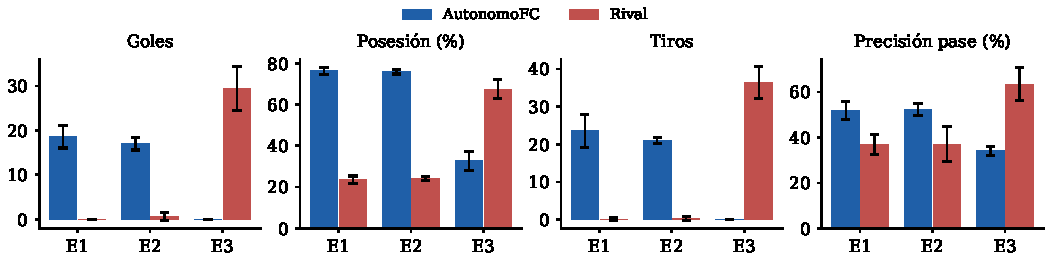
\includegraphics[width=\textwidth]{fig/resultados.pdf}
\vspace{-1.5em}
\caption{Métricas de equipo por experimento (media $\pm$ desviación estándar).}
\label{fig:res}
\vspace{-1em}
\end{figure*}

Frente a la línea base (E1, E2) AutonomoFC gana los 8 partidos, con 76\,\%
de posesión y el balón en campo rival el 81\,\% del tiempo de juego. Las
métricas casi no cambian al invertir los lados, lo que valida la
transformación de coordenadas. La gestión de estamina se refleja en la
estamina mínima media (unas 3900 unidades frente a 540 de BaselineChaser,
que agota a sus jugadores persiguiendo el balón). La precisión de pase es
solo moderada (52\,\%) porque el criterio cuenta como pase todo toque
seguido de otro jugador, incluidos despejes y conducciones largas.

Frente a HELIOS-base (E3) el equipo pierde los tres partidos (media
0--29.3), no logra ningún tiro y su precisión de pase cae al 34\,\%
frente al 64\,\% del rival. El filtro geométrico de pase seguro no anticipa
que los rivales se muevan hacia la línea de pase, y la defensa individual,
sin línea coordinada, deja espacios entre defensas. En lo interno, la
auto-localización tiene un error mediano de 0.12~m y P90 de 0.38~m sobre
todas las muestras de E1 (Fig.~\ref{fig:loc}), y cada decisión tarda en
promedio 0.1~ms (P99 $<1$~ms), muy por debajo del ciclo de 100~ms.

\begin{figure}[t]
\centering
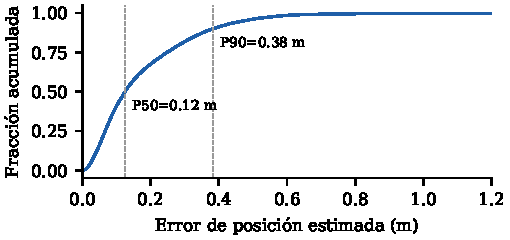
\includegraphics[width=\columnwidth]{fig/localizacion.pdf}
\vspace{-1.6em}
\caption{Distribución acumulada del error de auto-localización (E1, \LocN{}
muestras frente a la posición real del log).}
\label{fig:loc}
\vspace{-1em}
\end{figure}

\section{Video de demostración}
El video (\VideoDur{}) muestra, en el monitor oficial, la conexión de los 22
agentes, el saque inicial y fragmentos de E1 y E3 con rótulos de cada
experimento. Enlace público: \textbf{[pegar aquí el enlace de YouTube o
Google Drive]}.

\section{Errores y problemas encontrados}
\begin{enumerate}
\item \textbf{Configuración creada en un directorio literal ``\texttt{\textasciitilde}''}:
el servidor, ejecutado en el contenedor sin \texttt{HOME} expandido, creó
\texttt{./\textasciitilde/.rcssserver/}; se resolvió pasando todos los
parámetros por línea de comandos.
\item \textbf{Parámetro inexistente}: \texttt{server::random\_seed} no existe en
la versión 19; la semilla es \texttt{player::random\_seed}.
\item \textbf{Formato \texttt{see} v19}: los jugadores incluyen marcas
\texttt{k}/\texttt{t} (pateó/tackle) que rompían el parser numérico y
detenían a los 11 agentes; se filtraron y se protegió el bucle con manejo de
excepciones.
\item \textbf{Tiempo detenido}: en modos como \texttt{free\_kick\_fault} el
contador de ciclos no avanza; el agente solo respondía a ciclos nuevos, no
enviaba \texttt{(done)} y el servidor abortaba (``Waiting too long for
clients''). Ahora se decide en cada \texttt{sense\_body}.
\item \textbf{Arranque sin rival}: en modo sincrónico el
\texttt{connect\_wait} se consumía antes de que conectara el segundo equipo y
el partido comenzaba con un solo equipo; se elevó a 100\,000 ciclos.
\item \textbf{Orientación inestable}: al combinar el ángulo de cabeza de un
\texttt{see} viejo con el cuello actual, el cuerpo giraba sin control. Se
separó el ángulo del cuerpo y se integra el giro comandado.
\item \textbf{Doble patada}: tras patear, el modelo seguía viendo el balón en
el pie y pateaba otra vez; se actualiza la velocidad del balón con la patada
comandada.
\item \textbf{Compilación de HELIOS-base}: \texttt{librcsc} no detectaba
\texttt{netinet/in.h} con CMake ni instalaba todos los encabezados; se
corrigió \texttt{config.h} y se copiaron los encabezados.
\item \textbf{Faltas propias (E3)}: 7 \texttt{free\_kick\_fault}
(el que saca vuelve a tocar el balón, porque el bloqueo de 15 ciclos se
desactiva al pasar a \texttt{play\_on}) y 2 \texttt{back\_pass} (el
portero ataja pases de compañeros).
\item \textbf{Limitaciones abiertas}: el agente ignora los parámetros del
tipo heterogéneo asignado (velocidad, margen de pateo) y usa los del tipo~0;
la semilla del simulador no se puede fijar en la versión 19 (el parámetro
\texttt{random\_seed} está comentado en el código), así que los partidos no se
repiten exactamente y cada uno se trata como una muestra independiente.
\end{enumerate}

\section{Siguientes pasos}
\begin{enumerate}
\item Comunicación con \texttt{say}/\texttt{hear} (posición del balón e
intención de pase) para coordinar al interceptor y al receptor.
\item Intercepción con modelo de giro--carrera y velocidad del balón
filtrada (Kalman), y pase al espacio con predicción del receptor.
\item Estrategias de defensa colectiva: línea defensiva con trampa de fuera de
juego y presión al poseedor por dos jugadores.
\item Jugadas a balón parado (córner, saque de banda) y entrenador online
para asignar tipos heterogéneos.
\item Ajuste de parámetros (umbrales de pase/tiro, desplazamientos de la
formación) con búsqueda sistemática contra HELIOS-base, y torneo de al menos
20 semillas por configuración con intervalos de confianza.
\end{enumerate}

\begin{thebibliography}{9}
\bibitem{rcssmanual} M. Chen \emph{et al.}, ``RoboCup Soccer Server: Users
Manual,'' RoboCup Federation, 2003. [En línea]. Disponible:
\url{https://rcsoccersim.readthedocs.io}
\bibitem{rcssserver} RoboCup Soccer Simulator Maintenance Group,
``rcssserver,'' GitHub. \url{https://github.com/rcsoccersim/rcssserver}
\bibitem{rcssmonitor} RoboCup Soccer Simulator Maintenance Group,
``rcssmonitor,'' GitHub. \url{https://github.com/rcsoccersim/rcssmonitor}
\bibitem{helios} H. Akiyama y T. Nakashima, ``HELIOS Base: An Open Source
Package for the RoboCup Soccer 2D Simulation,'' en \emph{RoboCup 2013: Robot
World Cup XVII}, LNCS 8371, Springer, 2014, pp.~528--535.
\end{thebibliography}

\clearpage
\onecolumn
\appendices
\section{Código fuente}
El código completo se entrega también en \texttt{codigo\_fuente\_AutonomoFC.zip}.
Estructura: \texttt{agente/} (agentes y scripts de ejecución) y
\texttt{analisis/} (métricas). Ejecución: \texttt{./agente/run\_match.sh
runs/demo player.py AutonomoFC naive.py BaselineChaser}.
\begin{multicols}{2}
\lstinputlisting[language=Python,caption={agente/sexp.py}]{../agente/sexp.py}
\lstinputlisting[language=Python,caption={agente/world.py}]{../agente/world.py}
\lstinputlisting[language=Python,caption={agente/player.py}]{../agente/player.py}
\lstinputlisting[language=Python,caption={agente/naive.py}]{../agente/naive.py}
\lstinputlisting[language=bash,caption={agente/start\_team.sh}]{../agente/start_team.sh}
\lstinputlisting[language=bash,caption={agente/run\_match.sh}]{../agente/run_match.sh}
\lstinputlisting[language=Python,caption={analisis/metrics.py}]{../analisis/metrics.py}
\end{multicols}
\end{document}
